\documentclass[letterpaper, 11 pt, conference]{ieeeconf}  
\IEEEoverridecommandlockouts                             
\overrideIEEEmargins

\usepackage{graphics} % for pdf, bitmapped graphics files
\usepackage{epsfig} % for postscript graphics files
\usepackage{mathptmx} % assumes new font selection scheme installed
%\usepackage{times} % assumes new font selection scheme installed
\usepackage{amsmath} % assumes amsmath package installed
\usepackage{url}
\usepackage{amssymb}  % assumes amsmath package installed

\title{\LARGE \bf
Exploring the Space of Machine Learning Algorithms on Learning Stencil Based Kernels
}

\author{Sandesh Borgaonkar \& Vinu Joseph}% 
\begin{document}

\maketitle
\thispagestyle{empty}
\pagestyle{empty}

%%%%%%%%%%%%%%%%%%%%%%%%%%%%%%%%%%%%%%%%%%%%%%%%%%%%%%%%%%%%%%%%%%%%%%%%%%%%%%%%
\begin{abstract}
Abstract— Stencil based computations are used extensively in High Performance Computing (HPC) domain for finding
solutions of Partial Differential Equations (PDEs). These computations are represented in a polynomial form where the coefficients of the polynomial are influenced by the parameters such as boundary values, initial values, and the degree of accuracy. In this work, we present an empirical study to explore the solution space for following questions: i) is it possible to learn the coefficients of a given polynomial using regression analysis, and ii) how accurate the learning could be as compared to the original solution? And iii) what is the competitiveness of the various machine learning algorithms deployed for this purpose. Specifically, we use two state-of-the-art
machine learning packages, Libsvm and Liblinear, for learning the polynomial coefficients. In addition, we also implement our own version of learning model using stochastic gradient descent algorithm. Given the intractable size of the training data produced by the stencil kernels, we employ sampling strategy used in the prior work to reduce the sample size. We measure the effect of sample size on the quality of learning with respect to the three  different learning models described earlier.
\end{abstract}


%%%%%%%%%%%%%%%%%%%%%%%%%%%%%%%%%%%%%%%%%%%%%%%%%%%%%%%%%%%%%%%%%%%%%%%%%%%%%%%%
\section{INTRODUCTION}
Stencil based computations are an important area of study in the scientific domain. They find a variety of applications in areas such as solutions to Partial Differential Equations (PDEs) and related areas of scientific computation research. Stencil computations essentially are repeated update of neighboring points on a multidimensional grid, based on a given intial condition (initial value problem) or intial and boundary conditions (boundary value problem), and can be used to represent a wide variety of real world differential equations such as heat and wave propagations. The effort in this project was to learn the stencil points using the constituent grid points as features, and compare the performance of various learning algorithms on such a learning. If the study is successful, the results could be potentially utilized in a variety of applications that mandate computational optimizations on stencils. Also, the comparitive analysis could help in making informed choices over picking a given learning algorithm over others. For this project, the PDE we used was heat1d equation.

\section{THEORETICAL BASIS}
\subsection{Equation}
As shown in Fig.1, the evaluation of any given grid point on the stencil of the heat1d PDE can be represented as :\\ 
\begin{align*}
h[i+1,j] &=\alpha*h[i][j-1] +(2-\alpha)*h[i][j] \\
&\qquad +h[i][j+1] + h[i][j+1] + f[i][j]*dt
\end{align*}
\\
Here, $i+1$ is indicative of the time step for which the computation is being done, and $j$ is the $j_{th}$ discrete point that is being evaluated on the basis of $(j-1)_{th}$, $j_{th}$ and $(j+1)_{th}$ positions of the current time step $i$. The parameter $\alpha$ (also known as $cfl$) is defined by \\\\
\centerline{$\alpha = \dfrac{dt}{(dx)^2}$}\\

where $dt$ and $dx$ are the sizes of discretized time and length steps. Further, the term $f[i][j]*dt$ is the value of actual heat1d equation at point $(i,j)$ multiplied by the discretized time step $dt$.

\subsection{Initial and Boundary Conditions }
\textit{Initial condition} refers to the value of initial temperature of the rod element to be considered for heating. Such a condition is spread across the length of the rod, except for the end points. The temperature of the end points constitute the \textit{Boundary Condition}, which is imposed at every progressive time step of computation. We consider the following three initial condition variants : \\
\indent1. Triangular \\
\indent2. Sinusoidal \\
\indent3. Piecewise Linear \\

\begin{figure}
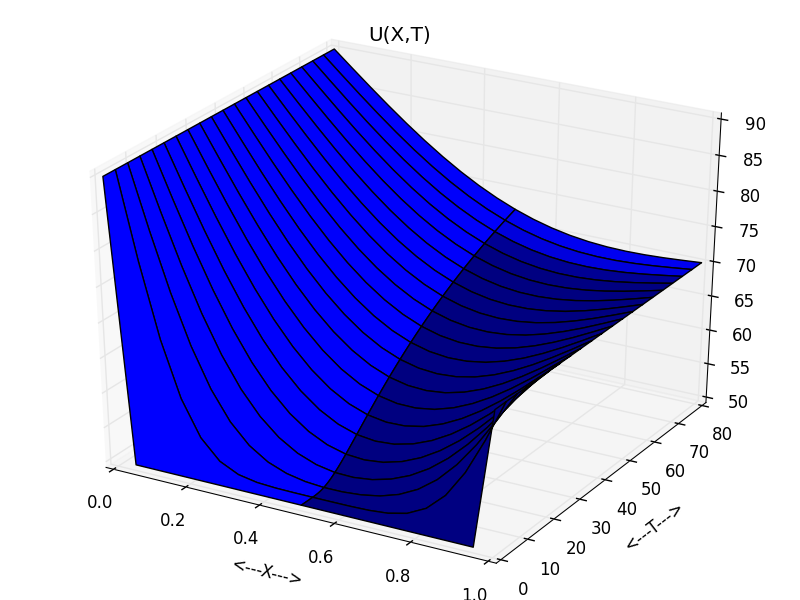
\includegraphics[scale=0.35]{plot_test_original_uni_1.png}
\caption{Uniform IC:50 and BC:90,70}
\label{uni1}
\end{figure}

\begin{figure}
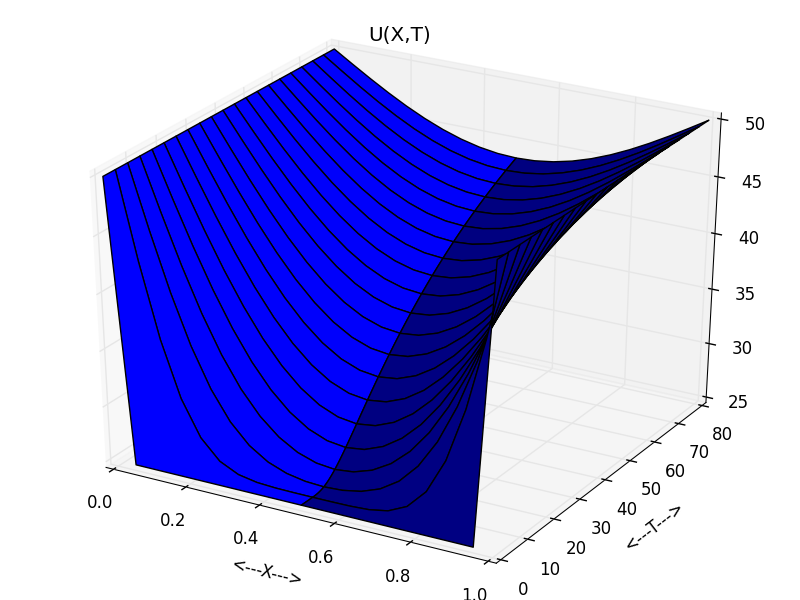
\includegraphics[scale=0.35]{plot_test_original_uni_2.png}
\caption{Uniform IC:25 and BC:50,50}
\label{uni2}
\end{figure}

\begin{figure}
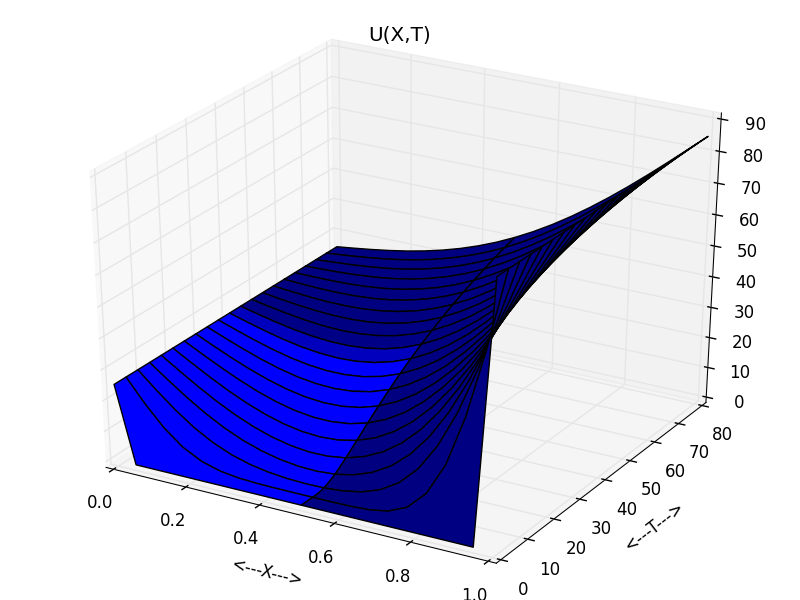
\includegraphics[scale=0.35]{plot_test_original_uni_3.png}
\caption{Uniform IC:0 and BC:25,80}
\label{uni3}
\end{figure}


\begin{figure}
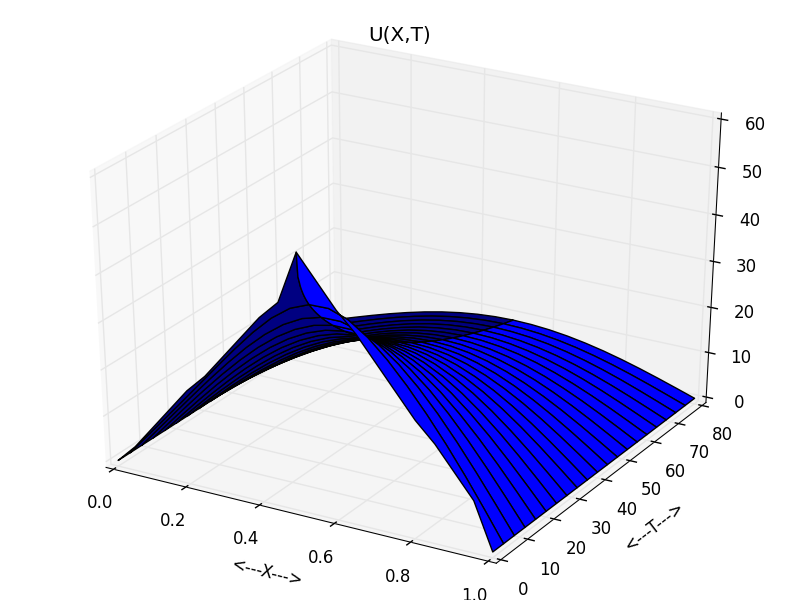
\includegraphics[scale=0.35]{plot_test_original_tri_1.png}
\caption{Triangular IC:70/(L/2)x and BC:0,0}
\label{tri1}
\end{figure}

\begin{figure}
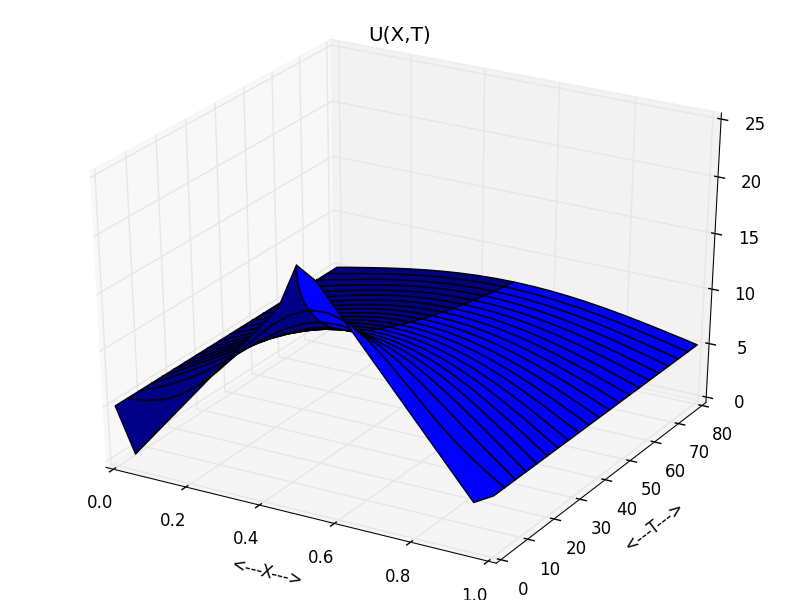
\includegraphics[scale=0.35]{plot_test_original_tri_2.png}
\end{figure}

\begin{figure}
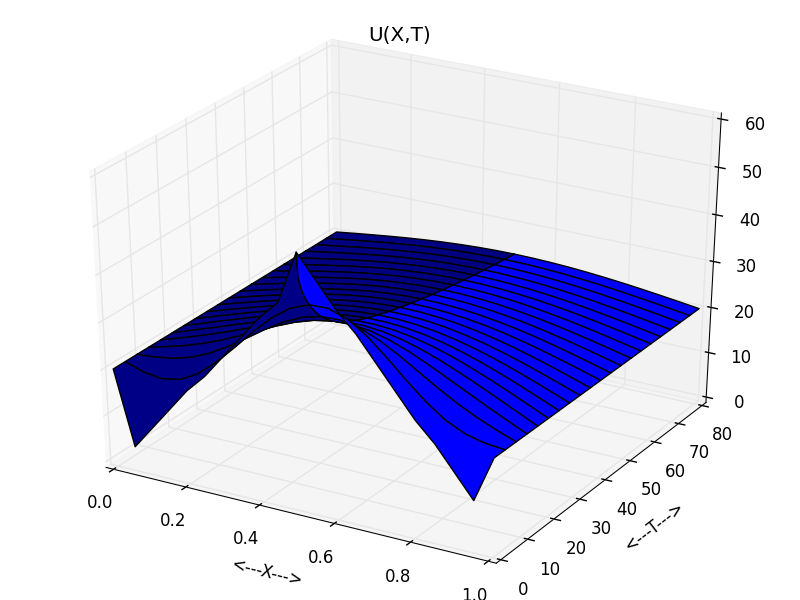
\includegraphics[scale=0.35]{plot_test_original_tri_3.png}
\end{figure}

\begin{figure}
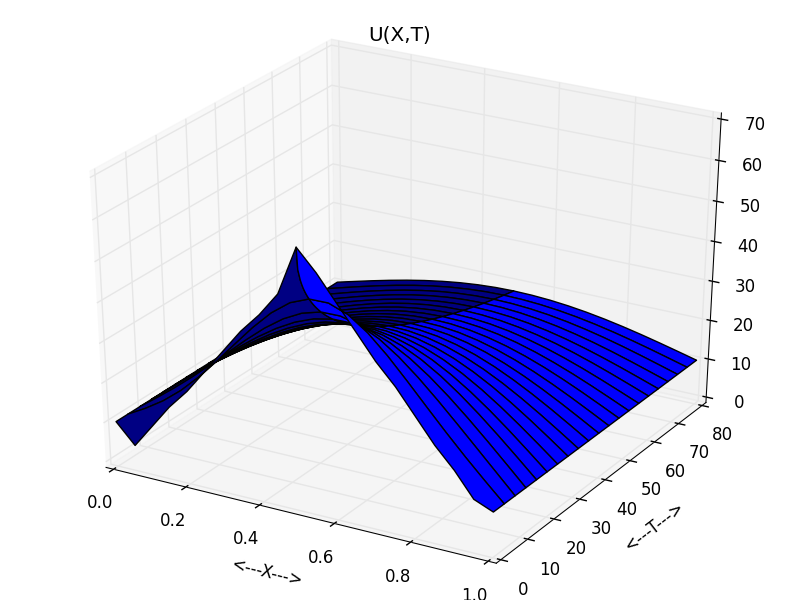
\includegraphics[scale=0.35]{plot_test_original_tri_4.png}
\end{figure}

\begin{figure}
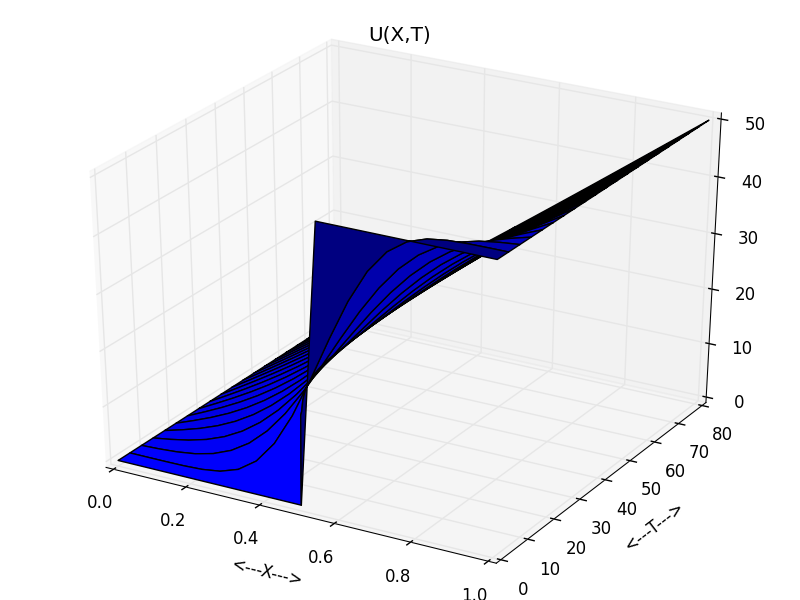
\includegraphics[scale=0.35]{plot_test_original_pwl_1.png}
\end{figure}
\begin{figure}
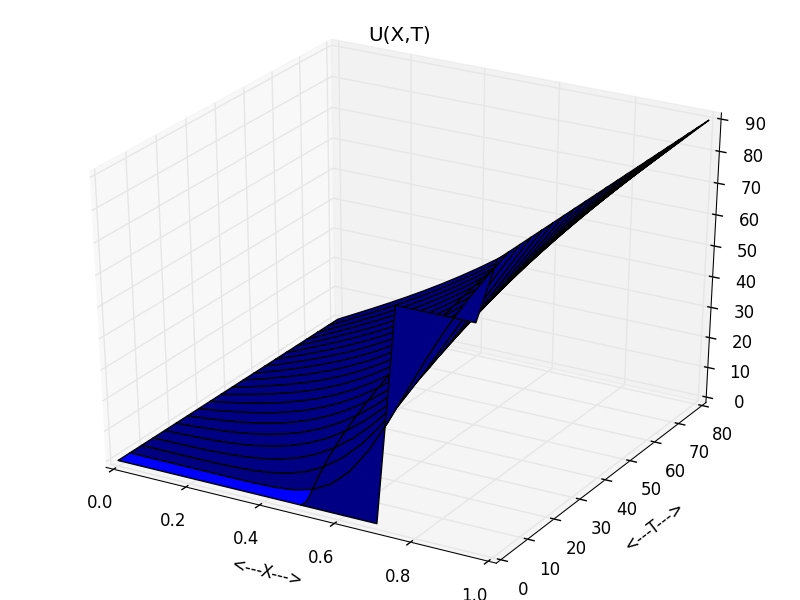
\includegraphics[scale=0.35]{plot_test_original_pwl_2.png}
\end{figure}
\begin{figure}
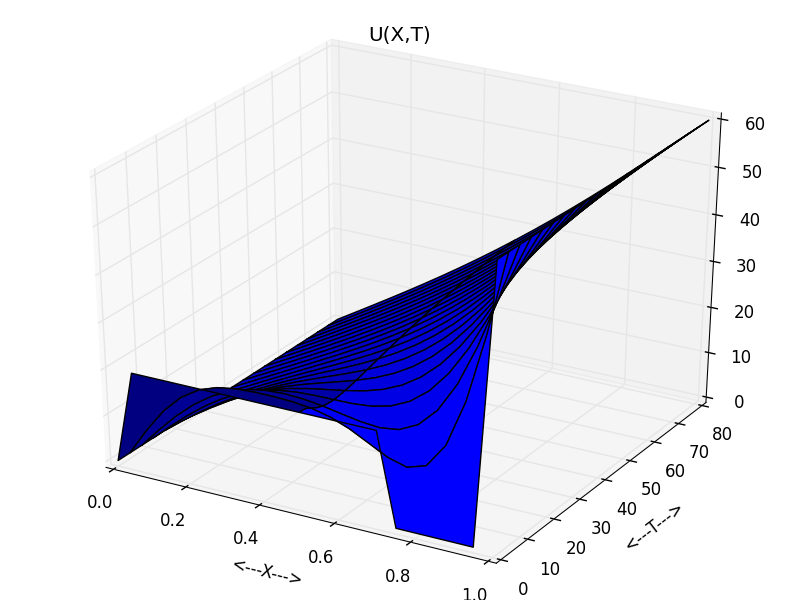
\includegraphics[scale=0.35]{plot_test_original_pwl_3.png}
\end{figure}

\begin{figure}
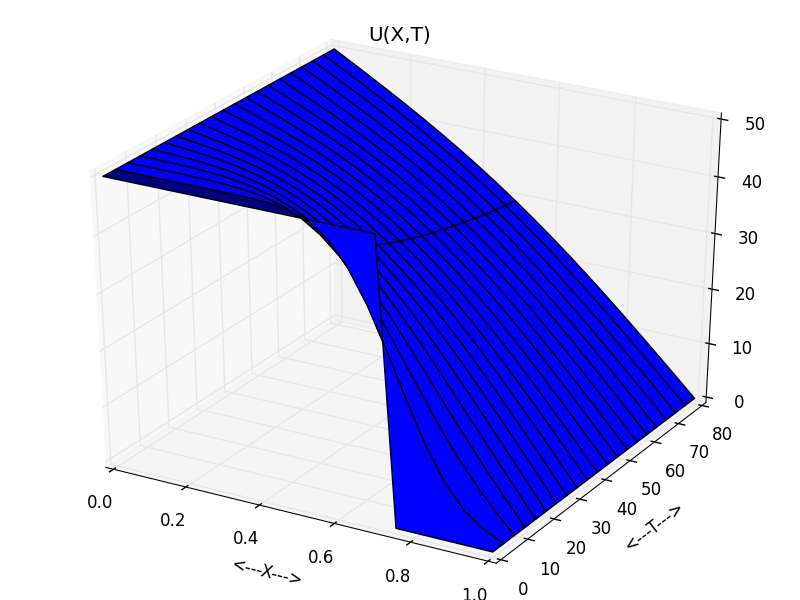
\includegraphics[scale=0.35]{plot_test_original_pwl_4.png}
\end{figure}

%TEST CASES
\begin{figure}
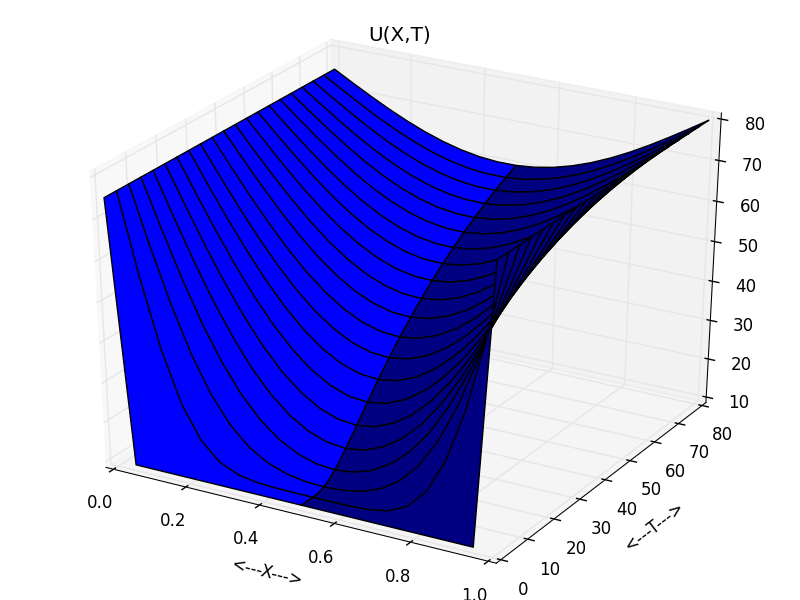
\includegraphics[scale=0.35]{plot_test_original_uni_4.png}
\end{figure}
while keeping the boundary conditions constant.
The goal of this project is to try to learn the computation of stencil points for heat1d stencil for a randomized set of initial condition, boundary condition, and discretized time steps $dt$ and $dx$, in order to learn weights that can be deployed towards computation of any heat1d stencil in general.  We deploy 3 learning algorithms - LibSVM, LibLinear and our own implementation of \textit{stochastic gradient descent} derived over an SVM objective, and also present a performance cross comparison of each of the algorithms used.

The following section decribes our experiments in detail. We try to outline the process of data collection, sampling, learning, cross validation and choice of hyper parameters, error collection finally the performance comparison of each of the algorithms used.  


\section{EXPERIMENTS}
\subsection{Data collection}
We collected the data by running the standard stencil program for heat1d \cite{c7} and listing the results in the standard LibSVM format. The collection comprised of results from multiple runs of the program over randomized sets of initial conditions, boundary conditions and the discretized sets of time and length steps. The same randomized set of inputs was repeated for each variant of initial conditions (i.e. Triangular, Sinusoidal and Piecewise Linear) to give us corresponding 3 sets of raw data collections (one for each variant).
\subsection{Sampling}
In this work, we employed the sampling approach described in \cite{c5}, where the  number of samples are tabulated for various confidence levels expressed as $(1-\delta)*100$\% and error $\epsilon$ . The work described in \cite{c2} provides pointers on information theoretic (entropy) based sampling, where a new sample from the population is added into the sample pool, based on how much variation it brings in into the training set.
\subsection{Choice of Parameters}
Cross validation experiment on each of the variants per algorithm (9cases), and the parameters finally chosen. 
\subsection{Learning}
Maybe show the weights reported in graphs?
\subsubsection{Using LibSVM}
3 variants
\subsubsection{Using LibLinear}
3 variants
\subsubsection{Using Our Implentation}
3 variants

\subsection{Test Error Analysis}
Deployment of the functions thus learned on the test set (9 cases again). Maybe show 3 plots, each for a variant with 3 lines for errors generated (bar graphs for training vs testing error)?
\subsubsection{Figures and Tables}

\section{Conclusion}


\addtolength{\textheight}{-12cm}   


%%%%%%%%%%%%%%%%%%%%%%%%%%%%%%%%%%%%%%%%%%%%%%%%%%%%%%%%%%%%%%%%%%%%%%%%%%%%%%%%
\section*{ACKNOWLEDGMENT}
%%%%%%%%%%%%%%%%%%%%%%%%%%%%%%%%%%%%%%%%%%%%%%%%%%%%%%%%%%%%%%%%%%%%%%%%%%%%%%%%

\begin{thebibliography}{99}

\bibitem{c1} Vishal C. Sharma, Ganesh Gopalakrishnan, Greg Bronevetsky, Detecting Soft Errors in Stencil based Computations

\bibitem{c2} 
Siamak Mehrkanoon, Johan A.K Suykens, Learning solutions to partial differcential equations using LS-SVM. 2015

\bibitem{c3}
Siamak Mehrkanoon, Johan A.K Suykens, LS-SVM approximate solutions to linear time varying descriptor systems, 2012

\bibitem{c4}
Eduardo Berrocal, Leonardo Bautista-Gomez, Sheng Di, Zhilling Lan and Frank Capello, Lightweight Silent Data Corruption Detection Based on Runtime Data Analysis for HPC Applications

\bibitem{c5}
Ken Kelly, Sample size planning for the coefficient of variation from the accuracy in parameter estimation

\bibitem{c6}
Richard H Byrd, Gillian M. Chin, Jorge Nocedal, Yuchen Wu, Sample Size Selection in Optimization Methods for Machine Learning

\bibitem{c7}
Burkardt, John, ”Scientific Computing Library” : \url{https://people.sc.fsu.edu/~jburkardt}

\bibitem{c8}
Kreyszig, Erwin.”Advanced engineering mathematics”. Wiley, 2011.

\bibitem{c9}
Vishal C Sharma, Approaches for Approximate Stencil based Computations

\bibitem{c10}
Rong-En Fan, Kai-Wei Chang, Cho-Jui Hsieh, Xiang-Rui Wang, Chih-Jen Lin, LIBLINEAR: A Library for Large Linear Classification , NTU

\bibitem{c11}
John burkardt, Florida State University, Codes and Data Sets \url{https://people.sc.fsu.edu/~jburkardt/py_src/fd1d_heat_explicit/}

\bibitem{c12}
Michael Bowles, Machine Learning in Python, Essential Techniques for Predictive Analysis

\bibitem{c13}
Bitbucket Repository \url{https://vinutah@bitbucket.org/ufmr/cs6350mlproj.git}

\bibitem{14}
Isaac Elias Lagaris, Aristidis Likas and Dimitirios I Fotiadis, Artificial Neural Networks for Solving ODE's and PDE's 

\end{thebibliography}



\end{document}
